\begin{figure}[ht]
    \centering
    \begin{tikzpicture}[
        ->, % directed edges
        >=stealth, % arrow tip
        node distance=3cm, % distance between nodes
        airport/.style={circle, draw, minimum size=2cm, font=\Large}, % style for airports
        flight/.style={font=\small} % style for flights
    ]

    % Nodes (Airports)
    \node[airport] (A) {SP \\ \faPlaneDeparture}; % São Paulo with departure icon
    \node[airport] (B) [right of=A] {RJ \\ \faPlaneDeparture}; % Rio de Janeiro with departure icon
    \node[airport] (C) [below of=A] {MG \\ \faPlaneDeparture}; % Minas Gerais with departure icon

    % Edges (Flights)
    \draw[->] (A) to node[flight, above] {\tikz[baseline]{\node[rotate=0]{\faPlane};}} (B); % Flight from SP to RJ, plane icon aligned (0 degrees)
    \draw[->] (B) to node[flight, right] {\tikz[baseline]{\node[rotate=220]{\faPlane};}} (C); % Flight from RJ to MG, plane icon rotated 270 degrees
    \draw[->] (C) to node[flight, left] {\tikz[baseline]{\node[rotate=96]{\faPlane};}} (A); % Flight from MG to SP, plane icon rotated 135 degrees

    \end{tikzpicture}
    \caption{Airports and Directed Flights}
    \label{fig:flight_network_graph}
\end{figure}
